\documentclass{report}
\usepackage{amsmath,amssymb,latexsym, mathtools}
\usepackage{verbatim}
\usepackage{algorithm}
\usepackage{changepage}
\usepackage{listings}
\usepackage{float}
\usepackage{color}
\usepackage{inconsolata}
\usepackage{parskip}
\usepackage{url}
\usepackage{enumerate}
\usepackage{geometry}
\usepackage{subcaption}
\usepackage{titlepic}

\newcommand{\nbody}{$N$-body}

\definecolor{mygray}{rgb}{0.5,0.5,0.5}
\renewcommand\arraystretch{2}
\raggedbottom

 \lstset{ %
  %backgroundcolor=\color{white},   % choose the background color; you must add \usepackage{color} or \usepackage{xcolor}
  basicstyle=\footnotesize\ttfamily\linespread{0.8},        % the size of the fonts that are used for the code
  breakatwhitespace=false,         % sets if automatic breaks should only happen at whitespace
  breaklines=true,                 % sets automatic line breaking
  captionpos=b,                    % sets the caption-position to bottom
  commentstyle=\color{mygray},    % comment style
  deletekeywords={...},            % if you want to delete keywords from the given language
  escapeinside={\%*}{*)},          % if you want to add LaTeX within your code
  extendedchars=true,              % lets you use non-ASCII characters; for 8-bits encodings only, does not work with UTF-8
  frame=single,	                   % adds a frame around the code
  keepspaces=true,                 % keeps spaces in text, useful for keeping indentation of code (possibly needs columns=flexible)
  keywordstyle=\color{black},   % keyword style
  lineskip={-0.7pt},
  otherkeywords={*,...},            % if you want to add more keywords to the set
  numbers=left,                    % where to put the line-numbers; possible values are (none, left, right)
  numbersep=5pt,                   % how far the line-numbers are from the code
  %numberstyle=\tiny\color{mygray}, % the style that is used for the line-numbers
  rulecolor=\color{black},         % if not set, the frame-color may be changed on line-breaks within not-black text (e.g. comments (green here))
  showspaces=false,                % show spaces everywhere adding particular underscores; it overrides 'showstringspaces'
  showstringspaces=false,          % underline spaces within strings only
  showtabs=false,                  % show tabs within strings adding particular underscores
  stepnumber=2,                    % the step between two line-numbers. If it's 1, each line will be numbered
  %stringstyle=\color{mymauve},     % string literal style
  tabsize=2,	                   % sets default tabsize to 2 spaces
  title=\lstname                   % show the filename of files included with \lstinputlisting; also try caption instead of title
}

\setlength\parindent{0pt}

\begin{document}
\lstdefinestyle{nonumbers}
{numbers=none}

\title{Final Project Report\\~\\
	\large Parallel Particle-Mesh Methods Applied to the \nbody{} Problem}
\author{Michael Whittaker (mjw297)\\Sheroze Sheriffdeen (mss385)}
\titlepic{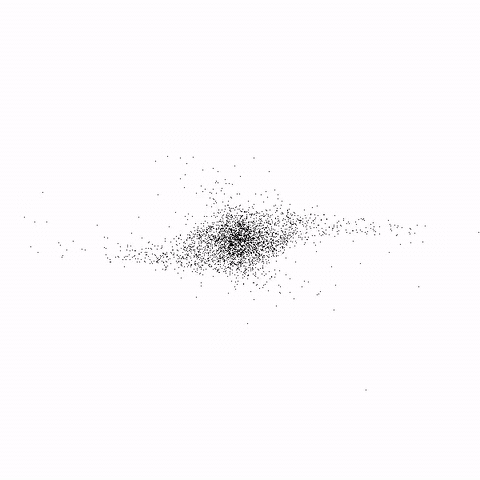
\includegraphics[width=0.7\textwidth]{./particles/9.png}}
\maketitle

\tableofcontents
%\begin{exercises}
%\item[]
\chapter{Introduction}
This final project explores parallel particle mesh methods applied to the collision-less \nbody{} problem in a shared memory programming model.

The \nbody{} system is a correlated dynamical system where each element can have a mass, radius, velocity, position and acceleration and each element is under the influence of a physical force, in our case, Newtonian gravity.

For the general \nbody{} problem with $n > 2$, barring selected configurations, the system cannot be solved analytically. To solve a system with $n > 2$, we create numerical models to approximate the evolution of the system with advancing time. Chapter~\ref{chap:models} introduces the physical and numerical models that enable us to simulate the behavior of bodies under the influence of gravity and discusses the performance and accuracy tradeoffs of the models.

Chapter~\ref{chap:impl} documents the implementation process of the simulation. The description and usage of the numerical libraries employed and the data marshaling and animation process.

Chapter~\ref{chap:perf} evaluates the performance of the system. The chapter analyzes the time profiles of the serial implementation and the parallel implementations, the strong and weak scaling properties of the parallel system and performance scaling with the number of particles and grid points.

Chapter~\ref{chap:sim} discusses a specific application of the \nbody{} simulator and the results of advancing a system of a large number of particles with time. This chapter introduces the correspondence between the simulation scales and the physical system and contains plots of the system evolution.

In conclusion, Chapter~\ref{chap:conc} mentions possible future work on the simulation and advanced numerical methods and parallelization schemes to further improve performance.


\chapter{Model Theory} \label{chap:models}

To simulate the \nbody{} problem, we have to employ models that enable us to track the attributes of the bodies of the system as we step forward in time. This section describes two such models and comments on their accuracy and performance tradeoffs.

\section{Particle-Particle Model} \label{sec:pp}
In class, we explored the three body problem, a specific case of the \nbody{} particle-particle model. At each time step of the system, the velocity, position and acceleration attributes of an element need to be updated according to the following set of equations.
\begin{align}
	\dfrac{\vec{v_i}}{dt} &= \dfrac{\vec{F}_i}{m_i} = G \sum_{j \neq i} m_j \dfrac{\vec{x}_j - \vec{x}_i}{\vert \vec{x}_j - \vec{x}_i \vert^3} \\
	\dfrac{\vec{x}_i}{dt} &= \vec{v}_i
\end{align}

\noindent
where $m_i$ is the mass of the $i^{\text{th}}$ particle and $G$ is the gravitational constant. Given the acceleration vector acting on a particle, we can then use a time integration scheme to solve the above coupled set of equations. In class, we used the automatic step Runge-Kutta method to update the position and velocity of each particle.

Although, this model provides good accuracy, the attributes modeled for a single element depend on every other elements in the system, leading to an algorithmic complexity of $O(n_p^2)$ where $n_p$ is the number of particles modeled by the system.

Therefore, for large number of particles we have to adopt a different model. Therefore, this project does not use the automatic stepsize Runge-Kutta method but further discussion of the method can be found in Chapter 17.2 of Numerical Recipes. \cite{numrecipes}

\section{Particle-Mesh Model}
In the particle-mesh approach, we exploit the force-at-a-point formulation and the field equation for the gravitational potential to compute a faster force calculation for the particles at the cost of accuracy. The space of interest is divided into a mesh and each particle is assigned to a mesh point depending on their location. The mesh sampling point defines the center of a cell.

\begin{figure}[H]
  \centering
  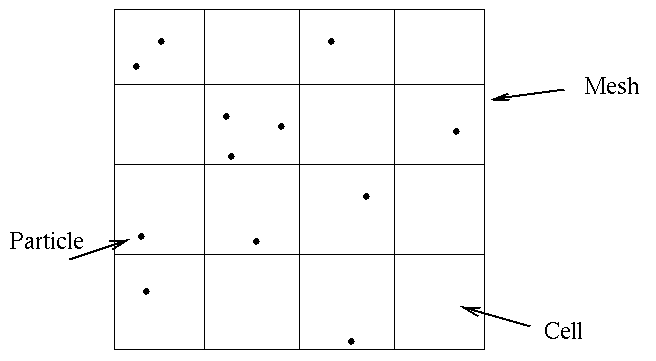
\includegraphics[scale=0.6]{pm_mesh.png}
  \caption{Particle-Mesh Model \cite{pm_mesh}}
   \label{fig:pm_mesh}
\end{figure}

\subsection{Physical Interpretation}

The gravitational field is defined at the center of a cell. Using the gravitational field at a mesh point, we can interpolate the force acting on a particle. To compute the gravitational field on a particle at a time step, we use Newton's law of universal gravitation:

\begin{equation}
	\dfrac{\vec{F}}{m} = \vec{g}
\end{equation}

The gravitational field $\vec{g}$ on a particle can be related to the gravitational potential $\phi$ by,

\begin{equation} \label{eq:phi_g}
	\vec{g} = - \nabla \phi
\end{equation}

and the potential $\phi(r)$ is related to the mass distribution by,

\begin{equation}
	\phi(r) = \dfrac{-Gm}{r}
\end{equation}

and obtaining the Poisson's equation for gravity:
\begin{equation}
	\nabla^2 \phi = 4\pi G \rho
\end{equation}

We can use Fourier analysis to solve the Poisson's equation for gravity. In Fourier space, the equation becomes,

\begin{equation} \label{eq:phi_k}
	k^2 \phi(\vec{k}) = 4 \pi G \rho(\vec{k})
\end{equation}

where $\vec{k}$ is the spatial frequency vector.

\subsection{Mass Density and the NGP scheme}

The mass density of the system is sampled at the cell centers of the mesh. To relate the masses of particles to the cell centers, a density assignment scheme is needed. The simplest method is the Nearest Grid Point (NGP) scheme.

\begin{equation}
	\rho_{i,j} = \dfrac{1}{(\triangle d)^2} \sum_{k=1}^{N_p} m_k \,
	\delta \left(\dfrac{x_k}{\triangle d} - i \right) \delta \left(\dfrac{y_k}{\triangle d} - j \right)
\end{equation}

where $\rho_{i,j}$ is the mass density at the cell $(i,j)$, $k$ iterates over the particles and $\triangle d$ is the sampling interval in space.

The following algorithm describes the 2 dimensional NGP scheme on a square mesh.

\begin{enumerate}
	\item For each particle $i$,
	\item $\quad$Find $(m, n)$, the index of the cell center in the mesh.
	\item $\quad$$\text{cell}_{\rho}(m,n) \leftarrow \text{cell}_{\rho}(m,n) + m_i$
	\item For each cell center $(m,n)$,
	\item $\quad$$\text{cell}_{\rho}(m,n) \leftarrow \text{cell}_{\rho}(m,n) / (\triangle d)^2$
\end{enumerate}

where $\text{cell}_{\rho}$ holds the mass density at the cell centers.

The NGP scheme provides a fast method to compute the mass distribution of the system since the core operation is a summation that is linear time on the number of particles. The disadvantage of the NGP scheme is that the mass densities are discontinuous.

\subsection{Gravitational Potential and Acceleration}
To solve for the gravitational potential $\phi$, we obtained equation~\ref{eq:phi_k}. Using the NGP scheme, we obtain the spatial distribution of density. Converting this density distribution to Fourier space, we obtain the relationship,

\begin{align}
	\phi(\vec{k}) &= \dfrac{ 4 \pi G \cdot \text{FFT}[ \rho(x,y) ]}{k^2}\\
	\phi(x,y) &= \text{FFT}^{-1} \left[ \dfrac{ 4 \pi G \cdot \text{FFT}[ \rho(x,y) ]}{k^2} \right]\\
\end{align}

where FFT is the Fast Fourier Transform. \cite{ngp} The implementation details of FFT is described in Section~\ref{sec:fftw}.

Then, using equation~\ref{eq:phi_g}, we can solve for the gravitational acceleration at a cell center using the central difference method:

\begin{align}
	g_x(i,j) &= - \dfrac{\phi(i+1,j) - \phi(i-1, j)}{2 (\triangle d)} \\
	g_y(i,j) &= - \dfrac{\phi(i,j+1) - \phi(i, j-1)}{2 (\triangle d)}
\end{align}

The gravitational acceleration of the cell centers can now be associated with the particles in the simulation using the NGP scheme.

\subsection{Particle-Mesh Algorithm Summary}

To summarize the particle-mesh method, the following algorithm describes a single time step:  \cite{csup}

\begin{enumerate}
	\item Assign mass to cell centers using the NGP scheme.
	\item Solve the Poisson's equation on the mesh in Fourier space by taking the Fourier transform of the mass distribution to obtain $\phi(\vec{k})$.
	\item Compute the inverse Fourier transform to obtain $\phi(x,y)$.
	\item Use central difference to obtain the gravitational acceleration at cell centers from $\phi(x,y)$.
	\item Use the NGP scheme to assign gravitational acceleration values to each particle.
	\item Use time integration to update the particle mass and velocity using the gravitational acceleration.
\end{enumerate}

\subsection{Performance and Accuracy tradeoffs}

The Particle-Particle model described in Section~\ref{sec:pp} although accurate requires a high computational cost, taking $O(N_p^2)$ time.

The advantage of the Particle-Mesh method is the performance. Updates to the particle attributes occur in $O(N_p)$ time. The slowest step in the method is the computation of the two dimensional Fourier transform which takes $O(N^2 log(N))$ time.

The increase in performance comes with an accuracy cost. Using the NGP scheme to compute acceleration on a particle decreases the resolution of the solver and to obtain fairly accurate time integration, the spatial sampling interval should be smaller than the wavelengths of importance in the physical system. Finer mass interpolation schemes such as CIC and mixed schemes are discussed in Hockney and Eastwood's Computer simulation using particles. \cite{csup}

\chapter{Implementation Details} \label{chap:impl}

\section{FFTW} \label{sec:fftw}

To compute the Fourier transform required in the Particle-Mesh method, we use the Fast Fourier Transform, obtained from the FFTW package. (www.fftw.org, the "Fastest Fourier Transform in the West" \cite{fftw}). In FFTW, the Discrete Fourier Transform of a complex one dimensional array $X$ computes $Y$ where,

\begin{equation}
	Y_k = \sum_{j=0}^{n-1} X_j e^{-2 \pi j k i /n}
\end{equation}

\subsection{Periodic Boundary Conditions}

The Discrete Fourier Transform assumes periodic boundary conditions. Therefore, our 2D gravitational potential is implemented with a toroidal geometry:

\begin{align}
	\phi(x+L,y) &= \phi(x,y) \\
	\phi(x,y+L) &= \phi(x,y)
\end{align}

where $L$ is the side length of the simulation in physical units. Therefore, any particle that goes out of the grid is 'wrapped around' and introduced from the opposite end.

\begin{lstlisting}[aboveskip=11pt,belowskip=-10pt]
if (particle_pos[2*i] < 0.0) particle_pos[2*i]     = fmod(particle_pos[2*i], L) + L;
if (particle_pos[2*i] > L) particle_pos[2*i]       = fmod(particle_pos[2*i], L);
if (particle_pos[2*i+1] < 0.0) particle_pos[2*i+1] = fmod(particle_pos[2*i+1], L) + L;
if (particle_pos[2*i+1] > L) particle_pos[2*i+1]   = fmod(particle_pos[2*i+1],L);
\end{lstlisting}

\subsection{FFTW Usage}
In the solution implementation $\texttt{serial.cpp}$, to compute the Fourier space representation of the density distribution $\rho$, we perform a forward transform.

\begin{lstlisting}[aboveskip=11pt,belowskip=-10pt]
fftw_plan rho_plan =  fftw_plan_dft_r2c_2d(N, N, rho, rho_k, FFTW_MEASURE);
fftw_execute(rho_plan);
\end{lstlisting}

which takes \texttt{rho}, that holds $N \times N$ 2D samplings of $\rho(x, y)$ and stores the Fourier space representation in \texttt{rho\_k}.

The function \texttt{fftw\_plan\_dft\_r2c\_2d} creates a plan that binds two arrays to perform an FFT operation. \texttt{r2c} variants of this function denotes a transform that goes from real numbers to complex numbers.

To compute  $\phi$, we perform the computation in equation~\ref{eq:phi_k} and use an inverse transform to obtain $\phi(x,y)$.

\begin{lstlisting}[aboveskip=11pt,belowskip=-10pt]
fftw_plan phi_plan =  fftw_plan_dft_c2r_2d(N, N, rho_k, phi, FFTW_MEASURE);
fftw_execute(phi_plan);
\end{lstlisting}

Since we perform this FFT operation for multiple time steps, FFTW offers an option to analyze the fastest style of computation for the compute by passing in the \texttt{FFTW\_MEASURE} flag to the function.

\section{Marshalling and Animations}

To visualize the \nbody{} simulation we marshal particle position data at each time step (implemented in \texttt{marshaller.cpp}) and use MoviePy \cite{moviepy} to create an MP4 representation of the simulation. Further information can be found in \url{https://github.com/sheroze1123/ppm} in \texttt{./scripts/mp4.py}

\chapter{Performance} \label{chap:perf}

\section{Design Decisions}

// Section to talk about our design decisions

\subsection{Vectorization}

// Vectorization report analysis, vectorized loops etc.

\subsection{OpenMP}

// I left the OpenMP intro here. You can leave it and just talk about the design decisions or we can get rid of it and go straight to design.

OpenMP (Open Multi-Processing) is an Application Programming Interface (API) that supports shared memory programming. The \nbody{} simulation using the particle mesh method decouples the particle attribute updates so that each particle's velocity and position can be independently updated using the shared resource, the array that holds the gravitational potential $\phi$.

The following example that updates the acceleration values in the $x$ direction highlights some of the useful directives in OpenMP.

\begin{lstlisting}[aboveskip=11pt,belowskip=-10pt]
#pragma omp parallel for
for (int j=0; j<N; j++) {
	for (int i=1; i<N-1; i++) {
		a_x[j*N + i] = (-phi[j*N + i-1] +  phi[j*N + i+1]) / scaling_factor;
	}
}
\end{lstlisting}

\begin{itemize}
\item \texttt{\#pragma omp} signifies that the current line is an OpenMP directive.
\item \texttt{parallel} clause creates a thread pool that enables multiple threads to perform operations on the shared memory \texttt{phi}.
\item \texttt{for} communicates to OpenMP that the following operation is a \texttt{for} loop to be executed in parallel.
\end{itemize}

\section{Timing Profiles}

// Let's talk about the Amplxe profiling here
\subsection{Serial Implementation}
\subsection{Parallel Implementations}

\section{Scaling Studies}

\subsection{Strong Scaling Study}

\subsection{Weak Scaling Study}

\subsection{Particle Scaling}

\subsection{Grid Size Scaling}

\chapter{Simulation Results} \label{chap:sim}

To see the \nbody{} simulation in action, we model a distribution of bodies with a mean mass of one solar mass around a massive object at the center.

\section{Conversion Units}

To scale the floating point numbers of the simulation, we adopt the following conversion units. \cite{conversion}

\begin{tabular}{| l | l |}
	\hline
	Simulation units & Physical units \\ \hline
	Time unit ($\triangle t$ = 1) & 1 year ($3.15 \times 10^7$ seconds)\\
	Space unit ($\triangle d$ = 1) & 1 AU ($1.4960 \times 10^{11}$ meters) \\
	Mass unit ($\triangle m$ = 1) & 1 solar mass ($1.9891 \times 10^{30}$ kilograms) \\ \hline
\end{tabular}

\section{Initial Conditions}

\subsection{Space distribution}

The total space of the simulation is $L$. The positions of the particles are randomly distributed according to a bivariate Gaussian distribution. The positions are sampled from the distributions,

\begin{align}
	p_x &= \dfrac{1}{\sqrt{2 \pi} \sigma} \exp{ -\frac{(x - \mu_x)^2}{2 \sigma^2}} \\
	p_y &= \dfrac{1}{\sqrt{2 \pi} \sigma} \exp{ -\frac{(y - \mu_y)^2}{2 \sigma^2}}
\end{align}

where $\mu_x = \mu_y = \dfrac{L}{2}$. This sampling produces particles that are centered around $\left( \dfrac{L}{2}, \dfrac{L}{2} \right)$ where a massive particle with mass $1000M_{\odot}$ lies. The bodies form a 'bulge' around the center of the configuration.

\subsection{Mass distribution}

Masses of the particles, excepting the central mass, are Poisson distributed with an expected value $\lambda$ of 1 solar mass.
\begin{equation}
	p_m = \dfrac{\lambda^k}{k!} e^{-\lambda} \quad\quad \text{where $k \in \{0, 1, 2, 3, \ldots\}$}
\end{equation}

\subsection{Velocity distribution}

The initial velocities of the particles are assigned assuming a stable circular orbit around the central mass neglecting the surrounding particles.
\begin{align}
	v_x &= -\sin(\theta) \sqrt{\dfrac{GM}{r}}\\
	v_y &= \cos(\theta) \sqrt{\dfrac{GM}{r}}\\
\end{align}

where $M$ is the mass of the central body, $G$ is the gravitational constant, $r$ is the separation between the central mass and the particle, and $\theta$ is the azimuthal angle between the central body and the particle body where the central body is at the origin. This provides the initial rotational component for the galaxy but does not create a stable configuration.

\subsection{Time Evolution Plots}

Given the initial conditions as described above, with simulation side length of $60$AU, 3000 particles, and a time step of $0.86$ hours, we advance the simulation and plot the resulting particle configuration at specific time intervals. The complete simulation can be found in \texttt{particles.mp4} or generated using \texttt{mp4.py}. The \texttt{README} file documents the simulation generation process.

\begin{figure}[H]
     	\centering
	\begin{subfigure}{.48\textwidth}
	\centering
     	\fbox{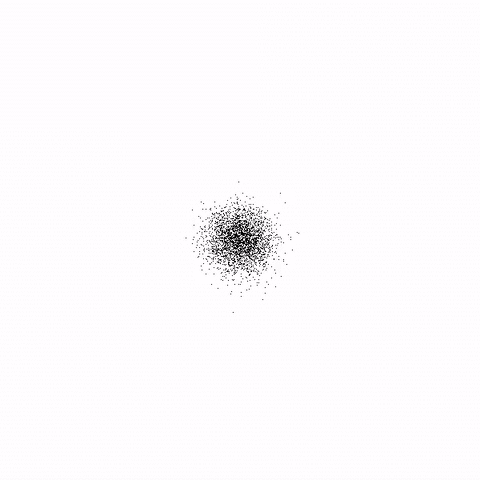
\includegraphics[width=0.95\linewidth]{./particles/0.png}}
	\caption{Bodies at $t = 0.0$ days, $L = 60$AU}
	\end{subfigure}
	\begin{subfigure}{.48\textwidth}
	\centering
     	\fbox{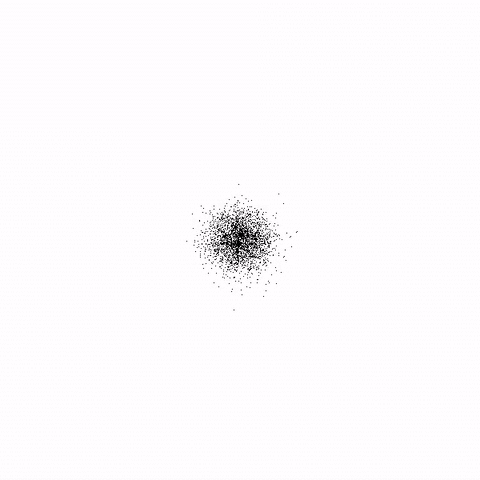
\includegraphics[width=0.95\linewidth]{./particles/1.png}}
	\caption{Bodies at $t = 2.43$ days, $L=60$AU}
	\end{subfigure}
	\begin{subfigure}{.48\textwidth}
	\centering
     	\fbox{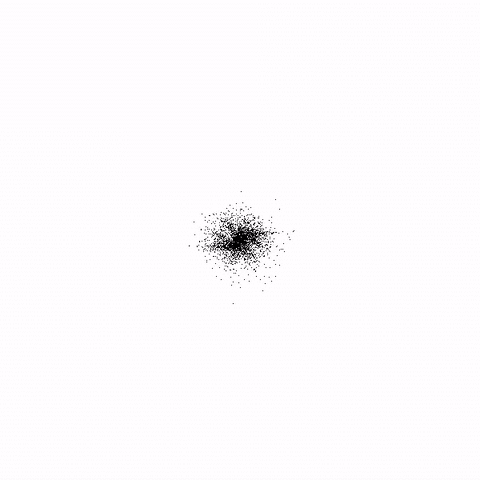
\includegraphics[width=0.95\linewidth]{./particles/2.png}}
	\caption{Bodies at $t = 4.86$ days, $L=60$AU}
	\end{subfigure}
	\begin{subfigure}{.48\textwidth}
	\centering
     	\fbox{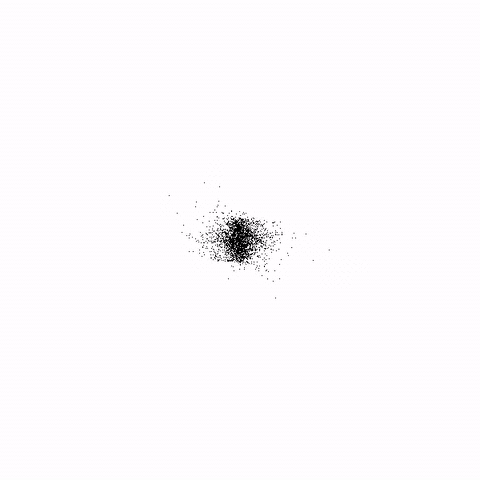
\includegraphics[width=0.95\linewidth]{./particles/4.png}}
	\caption{Bodies at $t = 7.3$ days, $L=60$AU}
	\end{subfigure}
	\caption{Configuration evolution with $\triangle t= 0.86$ hours, 3000 particles, $\mu_m = 1 \times 10^{30}$ kg}
	\label{fig:ev0}
\end{figure}

\begin{figure}[H]
     	\centering
	\begin{subfigure}{.48\textwidth}
	\centering
     	\fbox{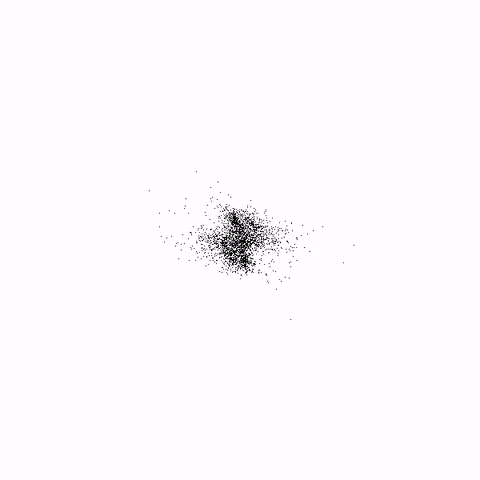
\includegraphics[width=0.95\linewidth]{./particles/5.png}}
	\caption{Bodies at $t = 9.73$ days, $L=60$AU}
	\end{subfigure}
	\begin{subfigure}{.48\textwidth}
	\centering
     	\fbox{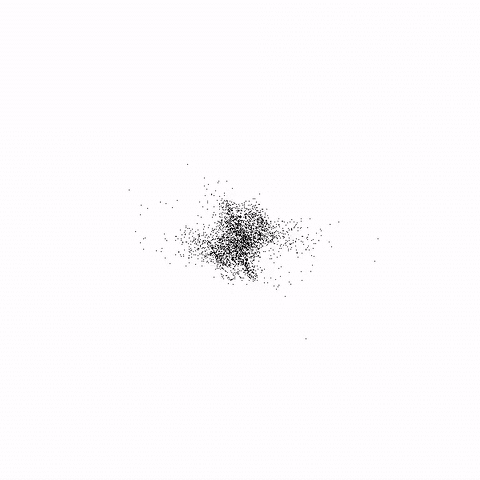
\includegraphics[width=0.95\linewidth]{./particles/6.png}}
	\caption{Bodies at $t = 12.16$ days, $L=60$AU}
	\end{subfigure}
	\begin{subfigure}{.48\textwidth}
	\centering
     	\fbox{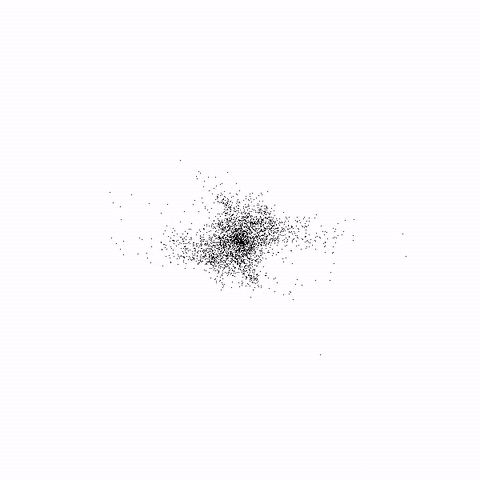
\includegraphics[width=0.95\linewidth]{./particles/7.png}}
	\caption{Bodies at $t = 14.6$ days, $L=60$AU}
	\end{subfigure}
	\begin{subfigure}{.48\textwidth}
	\centering
     	\fbox{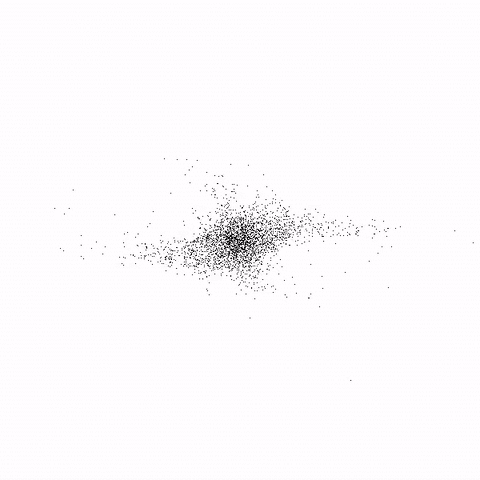
\includegraphics[width=0.95\linewidth]{./particles/8.png}}
	\caption{Bodies at $t = 17.03$ days, $L=60$AU}
	\end{subfigure}
	\caption{Configuration evolution with $\triangle t= 0.86$ hours, 3000 particles, $\mu_m = 1 \times 10^{30}$ kg}
	\label{fig:ev1}
\end{figure}

\begin{figure}[H]
     	\centering
	\begin{subfigure}{.48\textwidth}
	\centering
     	\fbox{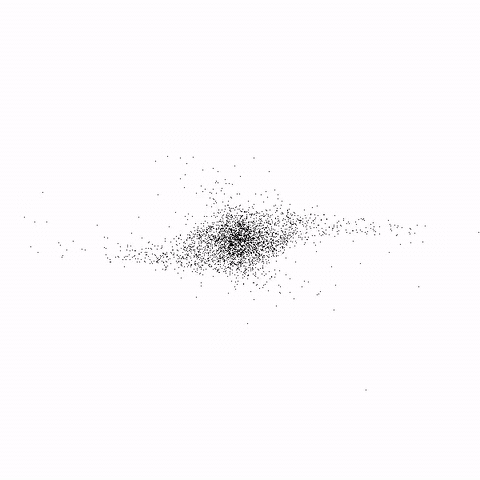
\includegraphics[width=0.95\linewidth]{./particles/9.png}}
	\caption{Bodies at $t = 19.46$ days, $L=60$AU}
	\end{subfigure}
	\begin{subfigure}{.48\textwidth}
	\centering
     	\fbox{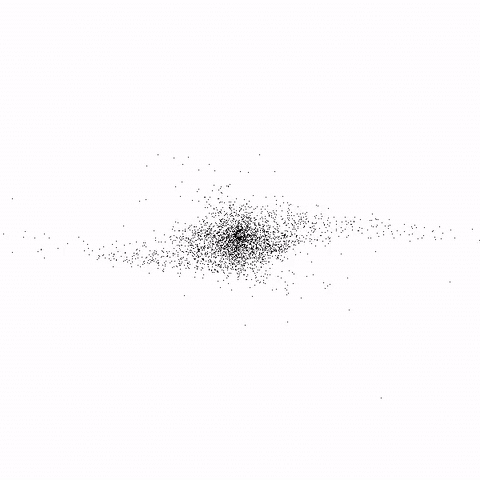
\includegraphics[width=0.95\linewidth]{./particles/10.png}}
	\caption{Bodies at $t = 21.9$ days, $L=60$AU}
	\end{subfigure}
	\begin{subfigure}{.48\textwidth}
	\centering
     	\fbox{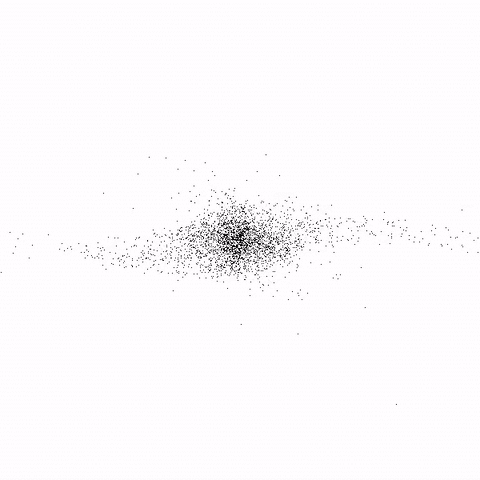
\includegraphics[width=0.95\linewidth]{./particles/11.png}}
	\caption{Bodies at $t = 24.33$ days, $L=60$AU}
	\end{subfigure}
	\begin{subfigure}{.48\textwidth}
	\centering
     	\fbox{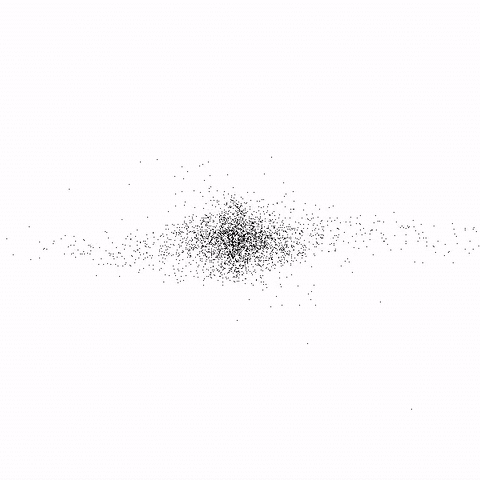
\includegraphics[width=0.95\linewidth]{./particles/12.png}}
	\caption{Bodies at $t = 26.76$ days, $L=60$AU}
	\end{subfigure}
	\caption{Configuration evolution with $\triangle t= 0.86$ hours, 3000 particles, $\mu_m = 1 \times 10^{30}$ kg}
	\label{fig:ev2}
\end{figure}

\chapter{Conclusions} \label{chap:conc}

// We can probably tailor this section to 5220 more

To improve the time integration process, future work can be undertaken to automatically scale the time step size to prevent instabilities. A maximum velocity can be enforced on the mesh, proportional to the cell widths, to limit the information propagation rate across the cells and the next time step can be dilated accordingly.

A better approximation for mass assignments to cells than the NGP scheme discussed here is the CIC method or the "cloud-in-cell" method described in Chapter 5-2-3 of Hockney and Eastwood's Computer simulation using particles. \cite{csup} It is costlier in terms of floating point operations per mass assignment run, but provides a more accurate estimate, giving forces continuous in volume. This method considers the closest $2^N$ neighbors where $N$ is the dimensionality of the problem, to assign masses.

The biggest shortcoming of the Particle-Mesh method is the low resolution of forces computed when particles are near each other. This arises from the regular discretization scheme and is proportional to the cell width $\triangle d$. To overcome this shortcoming, a possible numerical model is the P3M model. \cite{ngp} The Particle-Particle/Particle-Mesh model refines the mesh method by computing the pair-wise force interaction between particles if the distance between particles are below a certain threshold. P4M method is a parallel variant of the P3M and improves on the performance. \cite{p4m}

To scale the \nbody{} simulation to large values, a smarter scheme is needed that is able to distribute the computation across multiple computers. OpenMP, due to its shared memory programming model, does not provide this ability to scale. MPI (Message Passing Interface), is a programming model that enables us to perform computations in parallel on separate processors that can span multiple machines. FFTW offers an MPI variant of the FFT computation that can be used to explore the distributed computation model. \cite{fftw_mpi}

Finally, to improve the viewing experience of the simulation, we can invert the data generation process where a graphical user interface can poll simulation data in real time from a data server. The initial attempt at this server-client structure is documented in the Github page for the CS5220 final project under \texttt{scripts/fileserver.py} \cite{git}

\begin{thebibliography}{9}
\bibitem{numrecipes}
W. H. Press, S. A, Teukolsky, W. T. Vetterling and B. P. Flannery
\textit{Numerical Recipes, The Art of Scientific Computing, 3rd Edition}.
Camb. Univ. Press 2007.

\bibitem{csup}
R. Hockney, J. Eastwood, \textit{Computer simulation using particles} (Special student ed.). Bristol [England: A. Hilger.(1988)

\bibitem{dawson}
J. Dawson. \textit{Reviews of Modern Physics} 55, p.403 (1983)

\bibitem{pm_mesh}
M. Elmohamed (n.d.). \textit{N-Body Simulations}. Retrieved December 13, 2015, from http://www.new-npac.org/projects/cdroms/cewes-1999-06-vol2/cps615course/nbody-materials/nbody-simulations.html

\bibitem{ngp}
F. Vesely (n.d.). \textit{9.2 Particle-Mesh Methods (PM and P3M)}:. Retrieved December 13, 2015, from http://homepage.univie.ac.at/franz.vesely/simsp/dx/node48.html

\bibitem{fftw}
M. Frigo, S. G. Johnson, \textit{Design and Implementation of FFTW3}, Proc. of the IEEE, 93
(2005), p. 216-231.

\bibitem{moviepy}
\textit{User Guide}. (n.d.). Retrieved December 14, 2015, from https://zulko.github.io/moviepy/

\bibitem{conversion}
C. Mihos. (n.d.). \textit{Spiral Galaxies}. Retrieved December 14, 2015, from http://burro.case.edu/Academics/Astr222/equations.pdf

\bibitem{nbody_cmu}
\textit{N-Body/Particle Simulation Methods}. (n.d.). Retrieved December 14, 2015, from https://www.cs.cmu.edu/afs/cs/academic/class/15850c-s96/www/nbody.html

\bibitem{p4m}
P. Brieu, A. Evrard. (2000). \textit{P4M: A parallel version of P3M}. In New Astronomy (3rd ed., Vol. 5, pp. 163-180). Elsevier.

\bibitem{fftw_mpi}
\textit{Distributed-memory FFTW with MPI}. (n.d.). Retrieved December 14, 2015, from \url{http://fftw.org/doc/Distributed_002dmemory-FFTW-with-MPI.html}

\bibitem{git}
S. Sheriffdeen, M. Whittaker, (n.d.). \textit{Parallel Particle Mesh applied to \nbody{} simulations}. Retrieved December 14, 2015, from https://github.com/sheroze1123/ppm

\bibitem{vect}
Intel\textregistered  Xeon Phi\texttrademark Coprocessor - the Architecture. (n.d.). Retrieved December 14, 2015, from https://software.intel.com/en-us/articles/intel-xeon-phi-coprocessor-codename-knights-corner

\bibitem{openmp}
B. Barney (n.d.). \textit{OpenMP Tutorial}. Retrieved December 14, 2015, from https://computing.llnl.gov/tutorials/openMP/

\bibitem{astroparticle}
\textit{Solving the collisionless Boltzmann equation using \nbody{} simulations}. (n.d.). Retrieved December 14, 2015, from http://www.mi.infn.it/isapp04/Moore/notes2.pdf

\bibitem{simd}
G. Levand (n.d.). \textit{Chapter 2�Basics of SIMD Programming}. Retrieved December 14, 2015, from https://www.kernel.org/pub/linux/kernel/people/geoff/cell/ps3-linux-docs/CellProgrammingTutorial/BasicsOfSIMDProgramming.html
\end{thebibliography}

\end{document}
